\selectlanguage{italian}

Il Modello Standard della fisica delle particelle comprende il modello a quarks e il modello elettrodebole: quest'ultimo è stato introdotto a partire dallo studio delle violazioni di varie simmetrie.

\section{Simmetrie}

Oltre al modello a quarks, per mettere ordine nel particle zoo è necessario introdurre delle simmetrie che si osservano in varie reazioni.\\
Il concetto di simmetria in fisica delle particelle è stato introdotto da Weyl e Feynman: in generale essa è presente quando, a seguito dell'applicazione di una certa trasformazione ad un oggetto, esso rimane invariato; si parla di violazione di simmetria quando invece esso risulta modificato. Come messo in luce da Noether, il concetto di simmetria è estremamente importante in fisica poiché è legato alle leggi di conservazione di determinate quantità.\\
Il Modello Standard presenta naturalmente tre \textit{quasi-simmetrie}:
\begin{itemize}
	\item C-symmetry (carica): particella $ \mapsto $ antiparticella;
	\item P-symmetry (parità): $ \ve{r} \mapsto -\ve{r} $;
	\item T-symmetry (inversione temporale): $ t \mapsto -t $.
\end{itemize}
Queste sono dette quasi-simmetrie perché nell'Universo attuale ciascuna di esse è violata: ad esempio, l'interazione debole viola la C-symmetry e la P-symmetry (vedere esperimenti di Goldhaber e di Madame Wu), mentre il secondo principio della termodinamica asserisce che l'universo evolve in una direzione temporale ben precisa, violando la T-symmetry; inoltre, il decadimento dei kaoni neutri viola la CP-symmetry. Il Modello Standard, però, predice che la CPT-symmetry debba essere una simmetria: Ludens, Pauli e Schwinger (indipendentemente) hanno dimostrato che la Lorentz invariance implica la CPT-symmetry, dunque non c'è nessuna teoria consistente che permetta la violazione di tale simmetria. Una conseguenza della CPT-symmetry è che particelle e antiparticelle hanno stessa massa, stessa vita media e carica elettrica e momento magnetico uguali in modulo e di segno opposto.

\subsection{Esperimento di Madame Wu}

Nel 1956 Lee e Yang, con una literature review, notarono che i dati sperimentali non confermavano la P-symmetry nell'interazione debole. Rivolgendosi a Madame Wu, esperta di spettroscopia $ \beta $, proposero esperimenti per testare la P-symmetry nel decadimento $ \beta $.\\
L'esperimento di Madame Wu studia il decadimento $ \ch{^{60}Co} \rightarrow \ch{^{60}Ni}^* + e^- + \bar{\nu}_e $, con successiva emissione di $ 2\gamma $ per diseccitare il Nichel: gli osservabili sono dunque i fotoni e l'elettrone. In linea teorica, considerando un nucleo di cobalto nel suo rest-frame con spin $ \ve{s} $ e supponendo che l'elettrone venga emesso con momento $ \ve{p} $, l'operatore di parità agisce come $ \hat{\mathcal{P}} \ve{s} = \ve{s} $ e $ \hat{\mathcal{P}} \ve{p} = - \ve{p} $ (il momento angolare, essendo $ \ve{L} = \ve{r} \times \ve{p} $, è conservato dalla parità), dunque un modo per testare la P-symmetry è studiare la direzione d'emissione degli elettroni dal campione. In coordinate sferiche con $ \ve{s} \parallel \ve{e}_z $, basta studiare l'angolo d'emissione $ \theta $: l'operatore parità porta $ \theta \mapsto \pi - \theta $, dunque un'asimmetria nell'emissione dei elettroni dal campione agli angoli $ \theta $ e $ \pi - \theta $ indicherebbe una violazione della P-symmetry. Per quanto riguarda la distribuzione dei raggi $ \gamma $, essa è invariante per operatore di parità, poiché una volta fissato l'asse dello spin essa è determinata solo dal $ \Delta \ell $ della transizione (nel caso del $ \ch{^{60}Ni}^*(4^+) \rightarrow \ch{^{60}Ni}(0^+) $ sono due transizioni $ \Delta \ell = 2 $, dunque quadripolari).

\subsubsection{Apparato sperimentale}

\begin{figure}
	\centering
	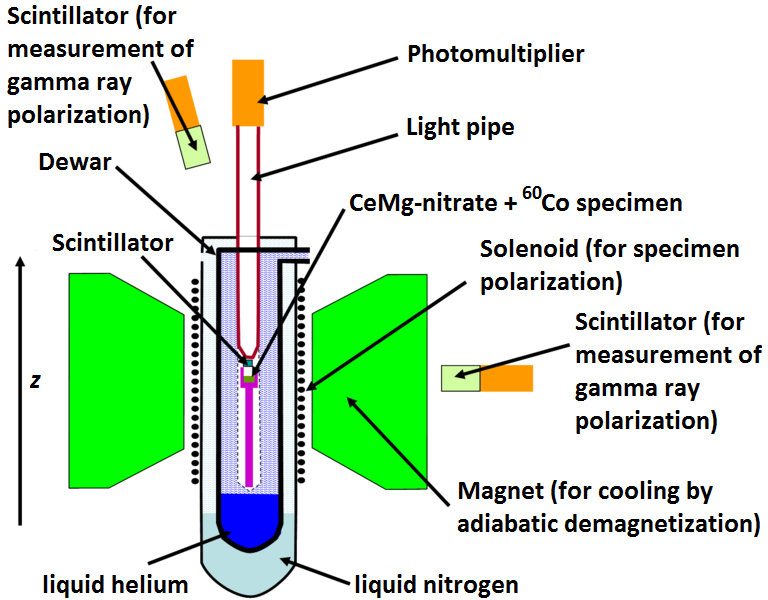
\includegraphics[width = 0.70\textwidth]{wu-exp.png}
	\caption{Madame Wu's experimental setup.}
	\label{wu-exp}
\end{figure}

L'apparato sperimentale di Madame Wu è schematizzato in Fig. \ref{wu-exp}. La sorgente di cobalto è inserita in misura opportuna per favorire il raffreddamento del sistema: infatti, una volta che il sistema è stato magnetizzato, per mantenere l'allineamento degli spin è necessario raffreddarlo a temperature di $ \sim 10\,\text{mK} $, poiché l'agitazione termica tende a rompere l'allineamento.\\
Per controllare che il sistema mantenga l'allineamento degli spin per un periodo sufficiente di tempo, sono presenti due scintillatori posti a 90° per monitorare la distribuzione dei raggi $ \gamma $: questa dipende dall'asse di spin, con una forte differenza di emissione tra il piano equatoriale e quello polare. Come si può vedere in Fig. \ref{wu-data}, il sistema mantiene correttamente la polarizzazione per circa $ 6 - 8\,\text{min} $.

\begin{figure}
	\centering
	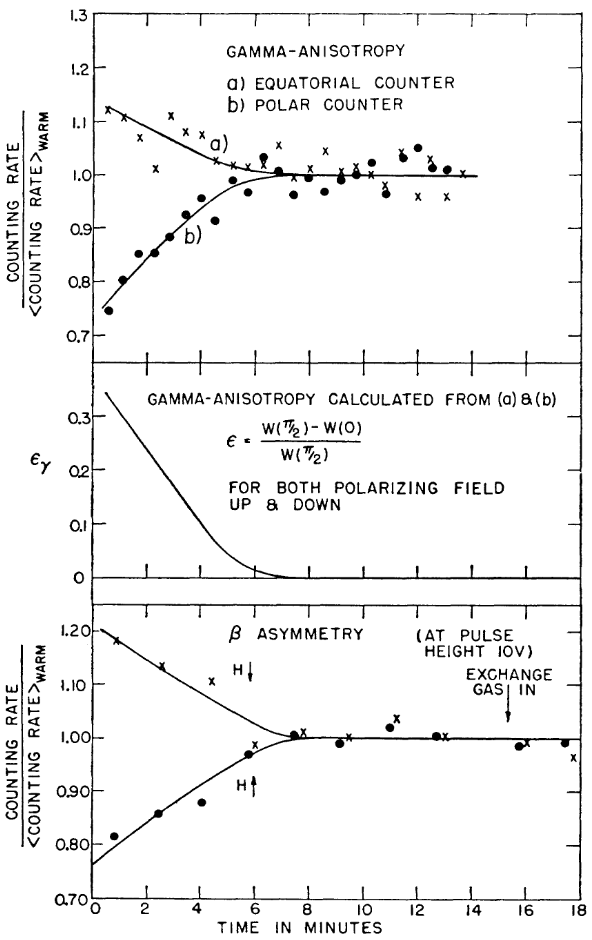
\includegraphics[width = 0.70\textwidth]{wu-data.png}
	\caption{Data from Madame Wu's experiment.}
	\label{wu-data}
\end{figure}

Sempre in Fig. \ref{wu-data} si può vedere che, per tutto il tempo in cui la direzione di riferimento data dagli spin polarizzati è ben definita, le distribuzioni di elettroni forward ($ \theta $) e backward ($ \pi - \theta $) sono decisamente asimmetriche: c'è una direzione preferenziale di emissione, che è quella backward rispetto alla direzione dello spin, dunque si evince che il decadimento $ \beta $ effettivamente viola la P-symmetry.

\subsection{Esperimento di Goldhaber}

A seguito dell'esperimento di Madame Wu sulla violazione della P-symmetry, nel 1957 Goldhaber mostrò che l'interazione debole violava anche la C-symmetry.\\
Innanzitutto, si definisce l'\textit{helicity} di una particella di momento $ \ve{p} $ e spin $ \ve{s} $ come:
\begin{equation}
	h \defeq \frac{\ve{s} \cdot \ve{p}}{\norm{\ve{s}} \norm{\ve{p}}}
	\label{eq:10.1}
\end{equation}
A seconda che il momento della particella sia parallelo o antiparallelo allo spin, l'helicity assume i valori $ +1 $ (right-handed) o $ -1 $ (left-handed). Inoltre, si vede che $ \hat{\mathcal{P}}h = -h $.\\
Con un esperimento molto sofisticato, Goldhaber riuscì a dimostrare che neutrini ed antineutrini hanno helicity differente. Per studiare un processo debole senza incorrere nel problema che il decadimento $ \beta $ è un decadimento a tre corpi, si considera la cattura elettronica che, essendo un processo a due corpi, permette di controllare energia e momento angolare e studiare le leggi di conservazione. In particolare, si consideri l'electron K-capture $ \ch{^{152}Eu}(0^-) + e^- \rightarrow \ch{^{152}Sm}^*(1^-) + \nu_e $, seguita da $ \ch{^{152}Sm}^*(1^-) \rightarrow \ch{^{152}Sm}(0^-) + \gamma $: essendo processi a due corpi, si ha $ E_{\nu_e} = 840\kev $ ed $ E_{\gamma} = 961\kev $. Si dimostra che $ h(\nu_e) = h(\ch{^{152}Sm}^*) = h(\gamma) $, dunque per trovare l'helicity del neutrino basta misurare quella del fotone. Quest'ultima è deducibile dal Compton scattering: la Compton cross-section dipende dall'orientazione relativa degli spin del fotone e dell'elettrone, ed in particolare si osserva un minor assorbimento se lo spin del fotone è parallelo a quello dell'elettrone. Dalle misure sperimentali di Goldhaber, si trova $ h(\nu_e) = -1.0 \pm 0.3 $, ovvero i neutrini sono sempre left-handed, mentre gli antineutrini sempre right-handed: di conseguenza, non c'è simmetria per scambio particella-antiparticella.

\subsection{Decadimento dei kaoni}

Il kaone neutro presenta un comportamento strano: esso infatti può decadere sia in due che in tre pioni, con tempi di decadimento molto diversi. Si parla di kaone short-lived $ K^0_S $, il quale decade come $ K^0_S \rightarrow \pi^+ \pi^- $ o $ K^0_S \rightarrow 2\pi^0 $ con $ \tau \approx 8.95\cdot10^{-11}\,\text{s} $, e di kaone long-lived $ K^0_L $, il quale decade come $ K^0_L \rightarrow \pi^+ \pi^- \pi^0 $ o $ K^0_L \rightarrow 3\pi^0 $ con $ \tau \approx 5.12\cdot10^{-8}\,\text{s} $.\\
Dato che i mesoni hanno sempre parità (intrinseca) negativa (quarks ed antiquarks hanno parità opposte), il decadimento del $ K^0_S $ è un'ulteriore dimostrazione della violazione della P-symmetry nei processi deboli.
Il decadimento del kaone neutro, però, può anche mettere in luce come l'interazione debole violi anche la CP-symmetry: con un esperimento del 1963, Cronin e Fitch dimostrarono che occasionalmente un kaone $ K^0_L $ può decadere in due pioni, violando anch'esso la P-symmetry.

\subsubsection{Esperimento di Cronin e Fitch}

L'esperimento consiste in un fascio di kaoni neutri in un tubo di $ 17\,\text{m} $, all'interno del quale vengono rilevati i pioni prodotti dal decadimento dei kaoni. Data la differenza di 3 ordini di grandezza nelle vite medie, ci si aspetterebbe di osservare soltanto i decadimenti a tre pioni del $ K^0_L $ all'estremità opposta del tubo: vengono invece osservati anche dei decadimenti a due pioni, con una frequenza di circa 1 ogni 500 decadimenti.\\
I decadimenti a doppio pione così osservati non sono attribuibili al decadimento del $ K^0_S $: data la half-life $ t_{1/2} = 5.5\cdot10^{-10}\,\text{s} $ ed assumendo $ v = 0.98c $, nel rest-frame la popolazione diventa $ 1/500 $ in appena $ 17\,\text{cm} $, ovvero $ 85\,\text{cm} $ nel frame del laboratorio ($ \gamma \approx 5 $); per qualsiasi velocità fisica, nessun $ K^0_S $ riesce a decadere all'estremità del tubo a $ 17\,\text{m} $.\\
L'unica spiegazione è dunque che in 1 decadimento ogni 500 il $ K^0_L $ decade in due pioni al posto di tre, violando dunque la CP-symmetry. Ciò può essere illustrato col modello a quarks: ricordando che $ \ket{K^0} = \ket{d\bar{s}} $ e $ \bar{K}^0 = \ket{\bar{d}s} $, si trova che:
\begin{equation*}
	\ket{K^0_S} = \frac{1}{\sqrt{2}} \left( \ket{K^0} + \ket{\bar{K}^0} \right)
	\qquad \qquad
	\ket{K^0_L} = \frac{1}{\sqrt{2}} \left( \ket{K}^0 - \ket{\bar{K}^0} \right)
\end{equation*}
Questi sono entrambi autostati di $ \hat{\mathcal{C}}\hat{\mathcal{P}} $, con rispettivi autovalori $ -1 $ e $ +1 $: si vede dunque che il decadimento del $ K^0_L $ secondo il canale del $ K^0_S $ viola la CP-symmetry.

\paragraph{Bariogenesi}

Il modello di bariogenesi proposto da Sakharov richiede la violazione della CP-symmetry per spiegare l'asimmetria tra materia ed antimateria, dunque lo studio di tale simmetria è di fondamentale importanza. Ad oggi, la violazione della CP-symmetry è stata osservata solo per l'interazione debole e non ci sono ancora evidenze che sussista anche per l'interazione forte.

\subsection{T-symmetry}

Data la violazione della CP-symmetry, se la CPT-symmetry deve sempre essere preservata, allora è necessario che i processi che violano la CP-symmetry violino anche la T-symmetry, ovvero che la probabilità del processo sia $ P(t) \neq P(-t) $.\\
Ad oggi, nessuna evidenza sperimentale di violazioni della T-symmetry è stata ancora osservata. Un esempio potrebbe essere la misura di un momento di dipolo elettrico non-nullo per il neutrone.

\subsubsection{Neutron electric dipole moment}

Il momento di dipolo elettrico del neutrone (nEDM), indicato con $ d_n $, dà un'indicazione sulle distribuzioni di cariche elettriche positive e negative all'interno del neutrone: in particolare, $ d_n \neq 0 $  indicherebbe che i centri di tali distribuzioni non coincidono. Ad oggi, la stima migliore non permette di dirimere la questione: $ d_n = (0.0 \pm 1.1) \cdot 10^{-26} e \, \text{cm} $.\\
Un momento di dipolo elettrico permanente nel neutrone violerebbe sia la P-symmetry che la T-symmetry: infatti, $ \hat{\mathcal{P}} d_n = - d_n $ e $ \hat{\mathcal{P}} \mu_n = \mu_n $, mentre $ \hat{\mathcal{T}} d_n = d_n $ e $ \hat{\mathcal{T}} \mu_n = - \mu_n $, dunque sia applicando $ \hat{\mathcal{P}} $ che applicando $ \hat{\mathcal{T}} $ si avrebbe una configurazione per $ d_n $ e $ \mu_n $ diversa da quella iniziale, violando la rispettiva simmetria.

\paragraph{Atomic EDM}

Un'alternativa per ricerche sulla violazione della T-symmetry è la ricerca di momenti di dipolo elettrico permanenti in nuclidi con deformazioni statiche permanenti (dunque non vibrazioni), in particolare nuclei con octupole deformations ($ \virgolette{pear-shaped} $). Negli anni sono stati individuati almeno tre nuclei pesanti con asimmetria rigida di carica ($ \ch{^{222}Ra} $, $ \ch{^{224}Ra} $ e $ \ch{^{226}Ra} $) e la ricerca al momento è incentrata sul come collegare tali misure a quelle di dipolo elettrico permanente nelle particelle.

\section{Modello elettrodebole}

Negli anni '50, a seguito della trattazione rigorosa dell'Elettrodinamica Quantistica (QED) e della formulazione da parte di Yang e Mills della teoria di gauge $ \SUn{2} $ per l'isospin, i fisici teorici iniziarono a notare una certa difficoltà nello svolgere i calcoli relativi all'interazione forte, dunque l'interesse si spostò sull'interazione debole: in particolare, si iniziò a pensare che ad alte energie l'interazione debole e quella elettromagnetica potrebbero essere unificate in un'unica \textit{interazione elettrodebole}.
Un'eventuale teoria elettrodebole, però, deve subire uno spontaneous symmetry breaking a basse energie, poiché i fotoni sono masless e con raggio d'azione infinito, mentre i bosoni che mediano l'interazione debole sono molto massivi ed a short range.

\subsection{Interazione debole}

Sperimentalmente, si trova che le dimensionless coupling constants delle interazioni del Modello Standard sono legate da:
\begin{equation}
	\alpha_s : \alpha_e : \alpha_w = 1 : 10^{-2} : 10^{-6}
	\label{eq:10.8454243}
\end{equation}
L'interazione debole può essere descritta tramite un modello a scambio di particelle, come le altre due interazioni. In particolare, essa è mediata da tre bosoni massivi di spin 1 (come il fotone, solo le proiezioni $ m_s = \pm 1 $ sono ammesse): $ W^{\pm} $ e $ Z^0 $. Sperimentalmente, questi sono stati osservati nel 1983 da Rubbia e van der Meer: essi sono bosoni estremamente massivi, con $ m_{W^{\pm}} = 80.4\gev/c^2 $ e $ m_{Z^0} = 91.2\gev/c^2 $. Di conseguenza, dato che il principio d'indeterminazione impone un range $ \Delta x \sim \frac{\hbar}{m c} $, si trova che l'interazione debole ha il range più corto tra le interazioni: $ \Delta x \sim 10^{-3} \fm $.\\
I tempi d'interazione sono più lunghi rispetto all'interazione forte: per i decadimenti deboli, si ha $ \tau \sim 10^{-8} - 10^{-13}\,\text{s} $. Inoltre, a differenza del bosone $ Z^0 $, i bosoni $ W^{\pm} $ possono cambiare il flavour dei quarks e leptoni con cui interagiscono: di conseguenza, l'interazione debole non conserva i numeri quantici associati alle generazioni di quarks (isospin, stranezza, etc.).\\
Un esempio di decadimento debole è il decadimento del neutrone $ n \rightarrow p e^- \bar{\nu}_e $: un quark down nel neutrone diventa un quark up, rendendo il nucleone un protone, emettendo un bosone $ W^- $ virtuale, il quale decade entro $ 10^{-18}\,\text{m} $ in una coppia elettrone-antineutrino elettronico: confrontando tale distanza con le dimensioni del nucleone, si può dire che il decadimento del bosone $ W^- $ avvenga praticamente nel punto d'emissione stesso.

\subsection{Teoria GWS}

Un modello di unificazione dell'interazione elettromagnetica e di quella debole fu proposto a fine anni '70 da Glashow, Salam e Weinberg. Nella teoria GWS, ad alte energie ($ \sim 100\gev $) l'interazione elettrodebole è mediata da quattro bosoni massless di spin 1; scendendo a basse energie, tre di questi bosoni acquistano massa per rottura spontanea di simmetria. Il processo di spontaneous symmetry breaking è legato all'\textit{angolo di Weinberg} (o weak mixing angle):
\begin{equation}
	\cos \theta_W \defeq \frac{m_{W^{\pm}}}{m_{Z^0}}
	\label{eq:10.2315454}
\end{equation}
Dai dati sperimentali, si trova $ \sin^2 \theta_W = 0.22305 $. Questo processo porta ad un coupling dei bosoni $ W^{\pm} $ e $ Z^0 $ col campo di Higgs (mediato dal bosone di Higgs, strength proporzionale alle masse), il quale è responsabile dell'acquisizione di massa delle particelle.

\subsubsection{Scoperta dei bosoni \texorpdfstring{$ W^{\pm} $}{TEXT} e \texorpdfstring{$ Z^0 $}{TEXT}}

Il valore dell'angolo di Weinberg fu misurato alla fine degli anni '70 in esperimenti di diffusione di neutrini ad alta energia, ricavando che la massa dei bosoni $ W^{\pm} $ e $ Z^0 $ doveva essere $ M \sim 80 - 90 \gev $. Per osservare particelle talmente massive, è necessaria un'energia al centro di massa $ E_{\text{cm}} \equiv \sqrt{s} $ ben al di sopra delle possibilità degli accelleratori esistenti all'epoca. In particolare, il protosincrotrone (SPS) del CERN (di cui Rubbia supervisionava il detector UA1), essendo un accelleratore a bersaglio fisso\footnote{Considerando una collisione $ p + N \rightarrow N' + X $, dove $ N,N' $ sono nucleoni ed $ X $ è la particella da produrre, la soglia di produzione è $ s = (p_p + p_N)^2 = (m_{N'} + M_X)^2 $ (pura massa, no energia cinetica). Per un collisore a bersaglio fisso $ p_p = (E_p,\ve{p}_p) $ e $ p_N = (E_N, \ve{0}) $, dunque:
\begin{equation*}
	s = (p_p + p_N)^2 = m_p^2 + m_N^2 + 2m_N E_p
	\quad \Rightarrow \quad
	E_p = \frac{(m_{N'} + M_X)^2 - m_p^2 - m_N^2}{2m_N} \sim \frac{M_X^2}{2m_p}
\end{equation*}
Per due fasci simmetrici, invece, $ p_p = (E_p,\ve{p}) $ e $ p_{N} = (E_p, -\ve{p}) $, quindi il valore di soglia è diverso:
\begin{equation*}
	s = (p_p + p_N)^2 = (E_p + E_N)^2 = 4E_p^2
	\quad \Rightarrow \quad
	E_p = \frac{m_{N'} + M_X}{2} \sim \frac{M_X}{2}
\end{equation*}
Con un collisore di fasci, a parità di energia del fascio, si producono energie nel centro di massa più elevate.}, avrebbe dovuto accelerare protoni a $ E_p > M^2 / 2m_p \approx 4000\gev $, un ordine di grandezza al di sopra del possibile.\\
Per questo morivo, Rubbia propose di convertire SPS in un anello di collisione protone-antiprotone, così da raggiungere le energie necessarie. La produzione di bosoni $ W^{\pm} $ e $ Z^0 $ in collisioni $ p\bar{p} $ avviene tramite il \textit{processo di Drell-Yan}: quando due adroni ad alte energie scatterano, una coppia quark-antiquark si annichila producendo un bosone virtuale, il quale a sua volta decade in una coppia leptone-antileptone. Esempi di reazioni possibili sono le seguenti:
\begin{equation*}
	u + \bar{d} \rightarrow W^+ \rightarrow e^+ + \nu_e
	\qquad
	\bar{u} +  d \rightarrow W^-\rightarrow e^- + \bar{\nu}_e
	\qquad
	u + \bar{u} \rightarrow Z^0 \rightarrow e^+ + e^- \,/\, \mu^+ + \mu^-
\end{equation*}
I decadimenti in due particelle sono utili poiché permettono di risalire all'energia della particella di partenza col metodo della massa invariante, anche se per quelli che involvono un neutrino vanno utilizzate altre tecniche.\\
Il problema di mantenere sotto controllo le dispersioni dei fasci di protoni ed antiprotoni fu risolto da van der Meer tramite lo \textit{stochastic cooling}: questa tecnica mantiene il fascio ben collimato tramite correzione automatica della traiettoria. In particolare, lungo l'anello sono poste due stazioni di controllo (pick-up probe e kicker): nella prima un sistema di rilevatori permette di misurare la posizione del fascio e la sua eventuale deviazione dalla traiettoria desiderata, inviando un segnale di correzione amplificato alla seconda stazione, la quale corregge la traiettoria.

\paragraph{Collisori di adroni e di leptoni}

Gli adroni, essendo più massivi, permettono di salire facilmente di energia nel centro di massa nei processi di scattering: gli accelleratori di adroni vengono usati principalmente per sondare settori inesplorati di energia per fare scoperte. D'altro canto i leptoni, non avendo struttura interna, permettono misure estremamente precise (sebbene ad energie minori) poiché si conosce perfettamente la particella incidente: gli accelleratori di leptoni servono dunque a misurare con precisione maggiore le proprietà delle particelle scoperte dagli accelleratori di adroni.

\paragraph{LHC e Higgs boson}

A seguito della scoperta dei bosoni mediatori dell'interazione debole, l'unica particella del Modello Standard non ancora scoperta era il bosone di Higgs. Per rilevarlo, sempre al CERN il LEP, in servizio fino al 2000, è stato riconvertito in un accelleratore di protoni, l'LHC, che ha permesso la scoperta del bosone di Higgs nel 2012. In particolare, lungo i $ 26.7\,\text{km} $ dell'LHC sono presenti quattro esperimenti: ATLAS e CMS, impiegati nella ricerca del bosone di Higgs, ALICE, per studi sulla materia nei tempi primordiali dopo il Big Bang, ed LHCb, per studi sulle particelle strane.










